\documentclass[12pt]{article}
\usepackage{graphicx}

\begin{document}
\begin{titlepage}
\begin{center}

\includegraphics[scale=1]{diagrams/up.png}
\\
\begin{huge}
\textbf{2017 Class Project}
\textbf{NavUP}\\
\end{huge}
\hfill \break
\begin{huge}
\begin{center}
\textbf{Team Broadsword}

\textbf{Testing Report}
\end{center}
\end{huge}
\hfill \break
\hfill \break
\begin{small}
	Bondjobo, Jocelyn 	13232852 \\
	du Plooy, Andries	15226183 \\
	Brijlal, Yashvir	14387744 \\
	Jones, Keanan		13036892 \\	
	Nxumalo, Banele		12201911 \\
	van Schalkwyk, John	14307317 \\
\end{small}

\end{center}
\end{titlepage}

\newpage
\pagenumbering{arabic}
\thispagestyle{empty}
\tableofcontents
\clearpage

\section{Test Model}

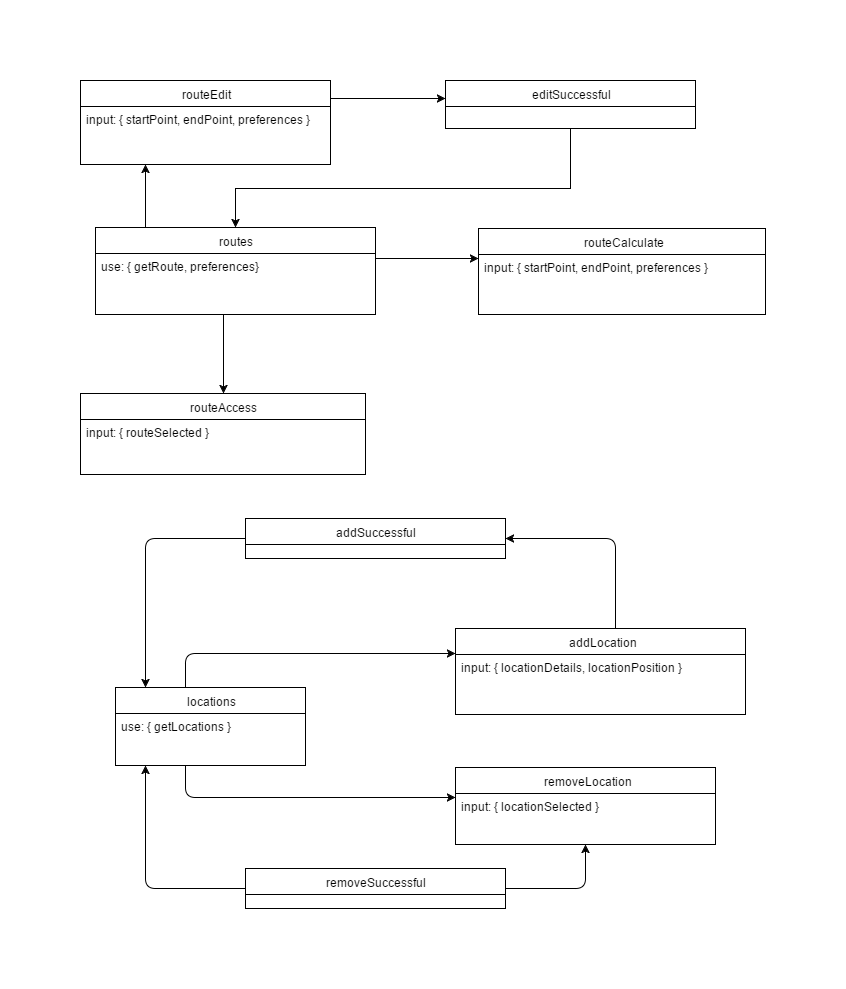
\includegraphics[scale=0.5]{diagrams/testModel.png}

\section{Service Contract Testing}

\subsection {Testing to get the route getRoute() - Getting and returning a route}
\begin{itemize}
\item 7/10
\item No parameters are accepted by the method in order to be able to test live data 
\item Test cases are generated, thus only test cases can be tested with a fixed response each time.
\item The method works, just not with live data.
\end{itemize}

\subsection{To modify a location modifyLocation() - Modify a location object}
\begin{itemize}
\item6/10
\item creates fixed and static location object
\item Not working with actual data
\item The method has no return or output. 
\item cannot test the output as there is no output or return
\end{itemize}

\subsection{addLocation(), removeLocation() - Adding and removing location objects}
\begin{itemize}
 \item 0/10
 \item Nothing in the function at all
 \item No logic present 
 \item void call
\end{itemize}

\subsection{modify route modifyRoute() - Changing existing route objects (Swap old route and the new route)}
\begin{itemize}
\item 1/10
\item No route has been tested 
\item Blank empty route object has been created instead.
\end{itemize}

\subsection{calculate route calculateRoute() - Calculate a new route between two locations}
\begin{itemize}
\item 1/10, The method structure was implemented, but always returns null.
\item Not return or displays nothing
\item Helper function called, calls another function that always returns null.
\end{itemize}

\subsection{Access Route - accessRoute() / saveRoute() / deleteRoute() / recordRoute()}
\begin{itemize}
\item 1/10
\item Tried to test function but nothing is coded.
\item No logic present, but test was included.
\end{itemize}

\section{Non-Functional Requirements}
\begin{flushleft}
Create a list of non-functional requirements tested, then evaluate each of these giving
a mark out of 10 and writing comments to justify the mark.
\end{flushleft}


    \begin{itemize}
        \item None given.
        \begin{itemize}
            \item 0/10
            \item No non-functional requirements were given or implemented. Thus there is nothing to test and no marks can be awarded
        \end{itemize}
    \end{itemize}
    
\section{Evaluation of test cases}
\subsection {LocationTest class}
\begin{itemize}
\item (2/10)
\item addLocation() method : Nothing implemented as test case 
\item modifyLocation() method: No reference to the actual object being modified
\item removeLocation() method: Nothing implemented as test case
\end{itemize} 

\subsection {NavigationHandlerTest class}
\begin{itemize}
\item (7/10)
\item addLocation() getRoute() method: not correctly implemented no handling of exceptions thrown
\item modifyLocation()accessRoute() method: working correctly
\item deleteRoute() method: working correctly
\item recordRoute() method: actual object created and recorded, working correctly
\item saveRoute() method: working correctly
\item modifyRoute() method: working correctly
\item calculateRoute() method: working correctly
\item safePreferences() method: current method implemented doesn’t receive parameter but a parameter is passed, method not working
\end{itemize}

\subsection {RoutesTest class}
\begin{itemize}
\item (5/10)
\item addRoute() method: working correctly
\item removeRoute() method: working correctly
\item getRoute() method: working correctly
\item search() method: Nothing implemented as test case
\item getRoutes() method: perfectly fine
\item modifyRoute() getPreferedRoute() method: nothing actually fetched as route
\item savePreference() method: because nothing stored unable to test this function
\item modifyRoute() method: seems to be working fine
\end{itemize}

\subsection {RouteTest class}
\begin{itemize}
\item (1/10)
\item getName() method: Nothing returned it is a void
\item calculateRoute() method: seems fine but no route returned it is a void
\item getLocations() method: seems fine but no Boolean returned it is a void
\end{itemize} 

\begin{flushleft}
The logic is present and some functions are implemented just that most of the methods are void so
currently no data returned, in other word all test cases should work which is not correct. Average mark
for this section is 4/10
\end{flushleft}

\end{document}